% Chapter 1

\chapter{Introduction} % Main chapter title

\label{Chapter1} % For referencing the chapter elsewhere, use \ref{Chapter1} 

\lhead{Chapter 1. \emph{Introduction}} % This is for the header on each page - perhaps a shortened title

%----------------------------------------------------------------------------------------

Energy prices, supply uncertainties, and most importantly environmental concerns (air and water pollution in particular) are driving the United States to restructure the US power contribution that are derived from various sources  and develop diverse sources of clean, renewable energy. The nation is working toward generating more energy
from domestic resources—energy that can be cost-effective and replaced or ``renewed" without contributing to
climate change or major adverse environmental impacts. In this context, solar energy and particularly wind energy (which is our current focus) has been one of the rapidly emerging and developing fields of research as a cleaner as well as safer alternative to energy sources from fossil fuels, natural gas and even nuclear energy. United States has a very rich resource of wind, with a mean spead peaking up to $\sim 9 \ m/s$ in central US (See Figure~\ref{fig:resource}). This has led to a strong and rapid growth in the mid-1980s followed by a short-term plateay during the electricity restructuring period in the 1990s and then regaining
momentum in 1999. Currently, the U.S. wind industry is growing rapidly, stimulated by policy incentives like sustained production tax credits (PTCs), rising concerns about climate change, and renewable portfolio standards (RPS) or goals in roughly
50\% of the states. With such growth rates and advancement in electrical power distribution and transmission technology , the Department of Energy (DoE) has set up a target of ``20\% Wind Scenario" which aims at producing 20\% of US Power from wind energy by the end of 2030. Under the ``20\% Wind Scenario", a
cumulative total of 7,600 million metric tons of $CO_2$ emissions would be avoided by 2030, and more than 15,000 million metric tons of $CO_2$ emissions would be avoided through 2050. This would potentially also reduce cumulative water consumption in the electric sector by 8\% (or 4 trillion gallons) from 2007 through 2030—significantly
reducing water consumption in the arid states of the interior West. In 2030, annual water consumption in the electric sector would be reduced by 17\%. With such targets and environmental incentives, the research scope of wind energy has expanded significantly over the last three decades, from a few KiloWatts being produced by single turbine to a hundreds of MegaWatts of power being produced by a large array of optimally placed wind turbines commonly referred to as ``wind farm" (See Figure~\ref{fig:figure_horns},~\ref{fig:onshore}).

In this context, we must mention that studying and optimizing the harvest of wind power using wind turbines is an extremely challenging task and thus it requires careful analysis of various aspects of wind turbines. While extensive amount of research has been performed in the field of wind turbines, there are several micro and macro aspects which demand a profound understanding. Studies in these domain are necessary not only for rudimentary reasons but also for the control and optimization required in the power generation process. Micro aspects would require understanding of various parts of the wind turbine, one of the most challenging research topic being the complex fluid flow around the dynamically moving wind turbine blades. The macro-effects would include understanding the multiscale turbulent transport phenomenon and counter-rotating wake dynamics downstream of wind turbine arrays and eventually of large wind farms containing multiple turbine arrays. Such studies are important from the fundamental fluid dynamic standpoint, since impingements of downstream wakes from one turbine on their next row counterpart affects the extraction of kinetic energy from the wind field which has a direct impact on electrical power generation.

For the macro-aspects of the studies in the wind energy domain, we propose to reconnoiter the multiscale turbulent flow dynamics of wind turbine arrays involving large length and time scales of motion. The interception of incoming turbulent flow field by the rotating turbines create counter-rotating wakes behind the turbines. The study of the dynamic behavior of the wakes in itself and their influence on the next row are essential in order to predict and optimize the performance of wind turbines arranged in a larger wind farm. Consequently, an efficient understanding of the wakes would require identification and analysis of some of the important parameters (e.g. yaw angle and turbine arrangement) of wake behaviour and then develop a fundamental understanding of the multiscale dynamics being affected by such parameters. In our current studies, the atmospheric boundary layer (ABL) flows approaching and surrounding the wind turbine are of extremely high Reynolds number ($Re \sim 10^8 - 10^{14})$. Consequently the stringent mesh requirements of direct numerical simulation (DNS) ($N_x\times N_y\times N_z \sim Re^{9/4}$) has rendered the method computationally infeasible for ABL flows~\cite{pope,chap,rey}. Large eddy simulation (LES) of wind turbine arrays is a promising technique with the potential of yielding a reliable data concerning the flow patterns as well as the energy output of turbines in a wind plant. An LES is justified for such calculations since it resolves the spatio-temporal evolution of large scale flow structures faithfully, which are the dominant contributors to the energy generated by wind turbine. Several attempts at characterizing the performance of wind turbine arrays with LES have been undertaken~\cite{ivanell,calaf,porte,churchfield, churchfield_2} in the last decade. \\
Additionally, for more than two wind turbines as is the case in large wind farms, a fully resolved calculation of the wind turbine blades is practically infeasible. Reduced-order aerodynamic models representing the effect of the rotating blades on the flow emerged and later evolved due to the computational bottleneck of fully-resolved calculations~\cite{rankine,glauert,ivanell,mikkelsen}. Actuator line (AL) model is the state-of-art reduced order model that has been used in the recent literature~\cite{mikkelsen,troldborg} and also been used in our current studies~\cite{peet2} in conjunction with LES of atmospheric boundary layer. It is important to note that most large scale wind farm simulations performed till date used low order methods and focused mainly on fully developed wind turbine array boundary layer (WTABL) using periodic boundary conditions~\cite{calaf,men2} with some studies emphasizing on large scale simulations with realistic turbulent inflow condition~\cite{porte2a,churchfield}. \\
The current computational problem we propose to do would involve several studies of massively parallel high $Re$ simulation of a $3\times 3$ wind turbine array using our spectral element AL model in atmospheric boundary layer to emulate the effects of large wind farm wake dynamics. Turbulent inflow conditions of wind turbine array simulations would be generated from our developed precursor atmospheric boundary layer simulation model involving near wall modeling in LES framework using higher order spectral element methods. The purpose behind the numerical tests is to understand the fundamental physics of wake developments in the wind turbines at extremely high Reynolds number and their effect on the turbines in the next row and beyond. This study retains its novelty in the focus and it is expected to elucidate more on design efficiencies of wind turbine arrays which are directly related to the optimization capabilities of power production and thrust generation in turbine blades.\\

However, it must be realised, that even though the fundamental studies of large wind turbine arrays have the capacity to extract information involving the interaction of the neutral ABL and wind turbine wakes, they have certain limitations. The neutral atmospheric boundary layer are numerically modelled from a single wind condition (mean wind flow direction is constant: streamwise direction) which at extreme cases might be quite far from realistic wind flows, which not only have spatio-temporal fluctuations of wind magnitude as in turbulence, but random variations in the wind direction (See Figure~\ref{fig:windir}).
 The ultimate larger goal of our work would involve incorporating data assimilation techniques to couple experimental field data obtained from LIDAR scans, to force realistic  atmospheric flows past wind turbine arrays. This has been further discussed in the Future Work section of the prospectus.
 \begin{figure}[h!]
\centering
        \begin{subfigure}[h]{0.5\textwidth}
                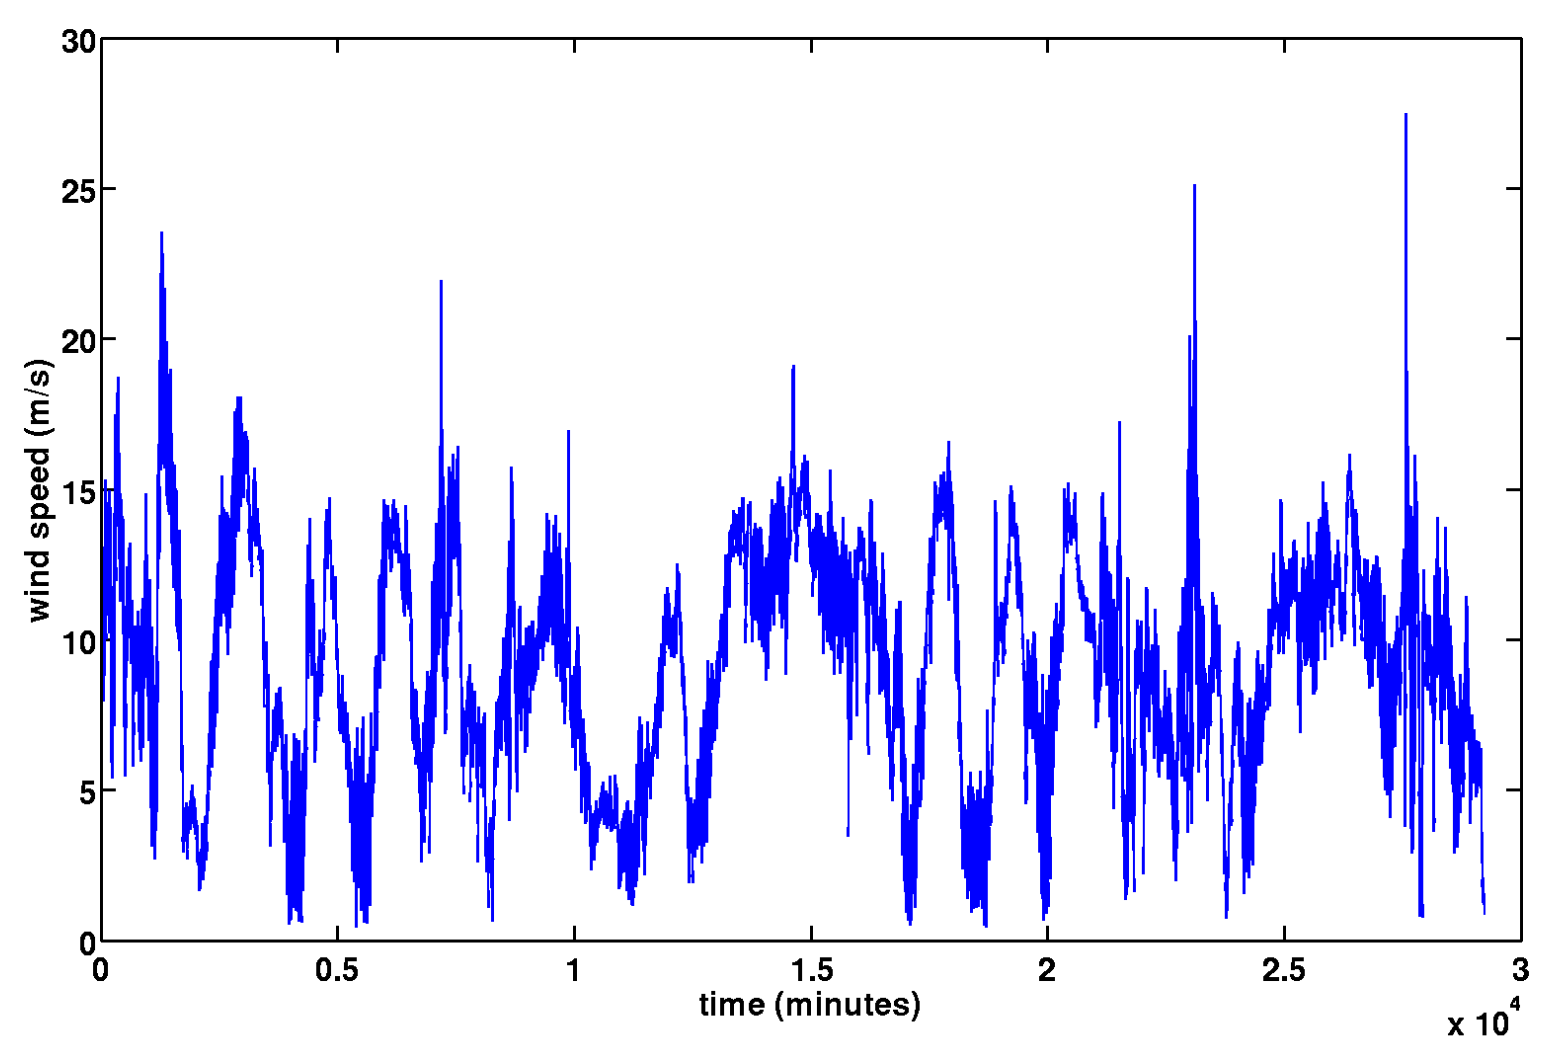
\includegraphics[width=\linewidth]{wind_mean.png}
                \caption{}
                \label{fig:figure_mean}
        \end{subfigure}%
        \centering
        \begin{subfigure}[h]{0.5\textwidth}
                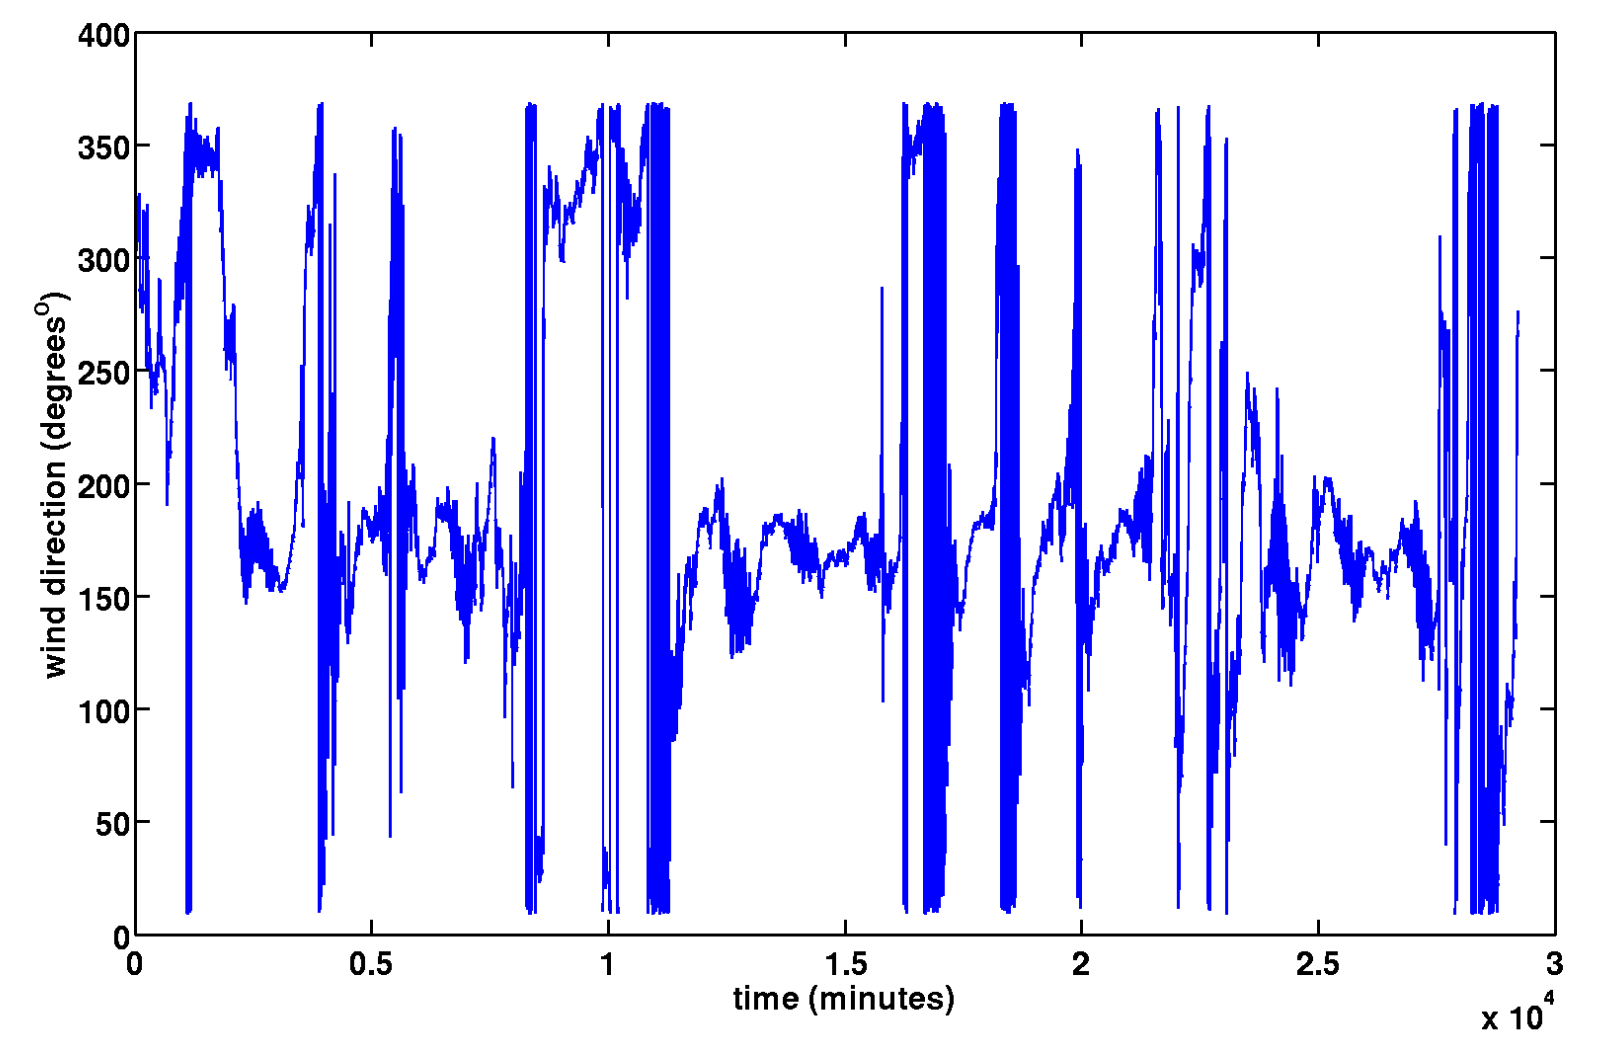
\includegraphics[width=\linewidth]{wind_direction.png}
                \caption{}
                \label{fig:dir}
        \end{subfigure}
       \caption[Wind speed and direction]{(A) Wind speed magnitude vs time    (B) Wind direction vs time, at a height of 50 m from the ground}\label{fig:windir}
\label{fig:smag}
\end{figure}
 
\begin{figure}[h!]
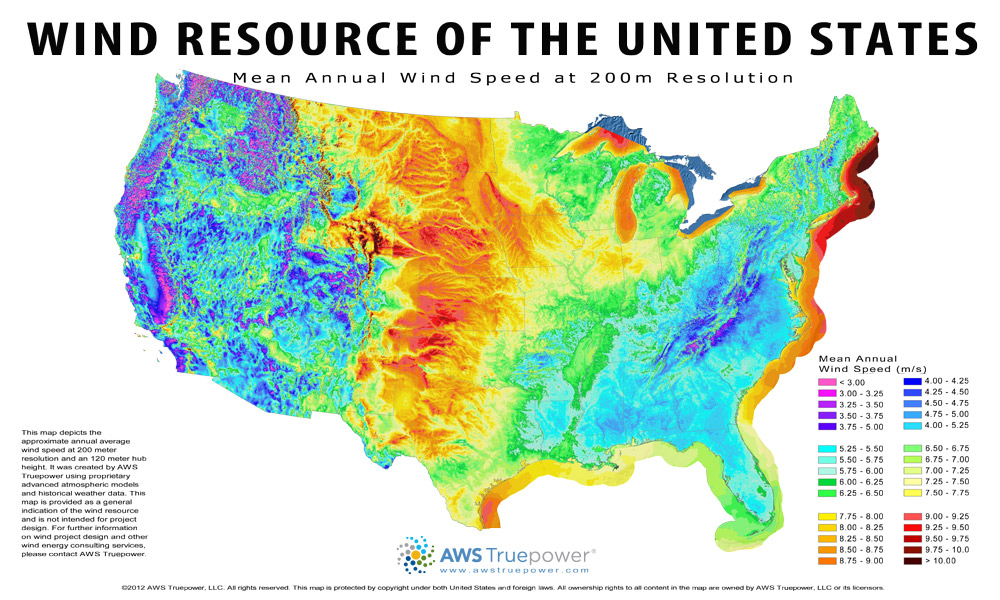
\includegraphics[width = 1.0\linewidth]{wind_us.jpg}
\caption[Mean annual Wind Speed]{Mean annual Wind Speed in different states of US. Courtesy: AWS Truepower}
\centering
\small source by:\url{https://www.awstruepower.com/} \label{fig:resource}
\end{figure}

\begin{figure}[h!]
\centering
        \begin{subfigure}[h]{0.5175\textwidth}
                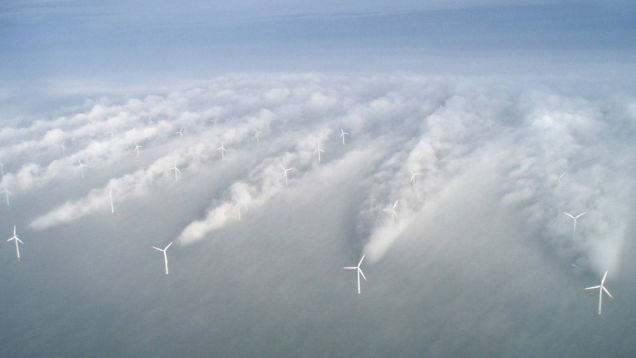
\includegraphics[width=\linewidth]{horns_rev.jpg}
                \caption{}
                \label{fig:figure_horns}
        \end{subfigure}%
        \centering
        \begin{subfigure}[h]{0.48675\textwidth}
                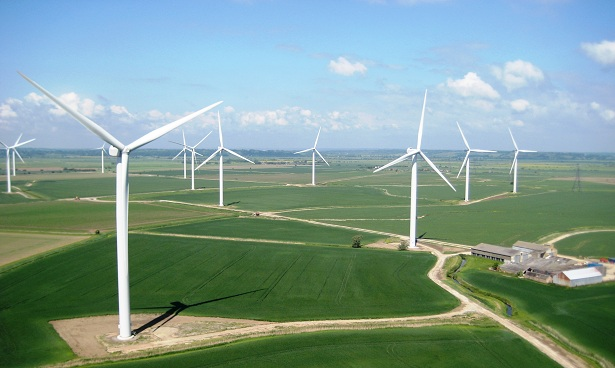
\includegraphics[width=\linewidth]{wind_onshore.jpg}
                \caption{}
                \label{fig:onshore}
        \end{subfigure}
       \caption[Offshore and Onshore wind farms]{(A) Offshore wind farm at Horn-Rev depicting wind turbine wakes (B) A classical Onshore wind farm}
\label{fig:smag}
\end{figure}

\begin{figure}[t!]
       \centering
        \begin{subfigure}[h]{0.5\textwidth}
                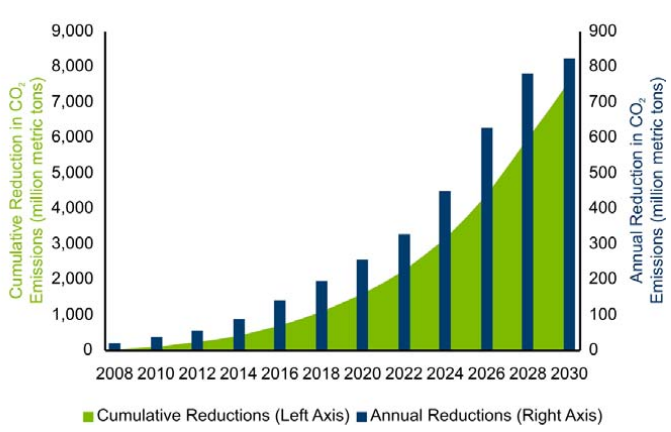
\includegraphics[width=\linewidth]{doe3.png}
                \caption{}
                \label{fig:do3}
        \end{subfigure}%
       \begin{subfigure}[h]{0.6\textwidth}
                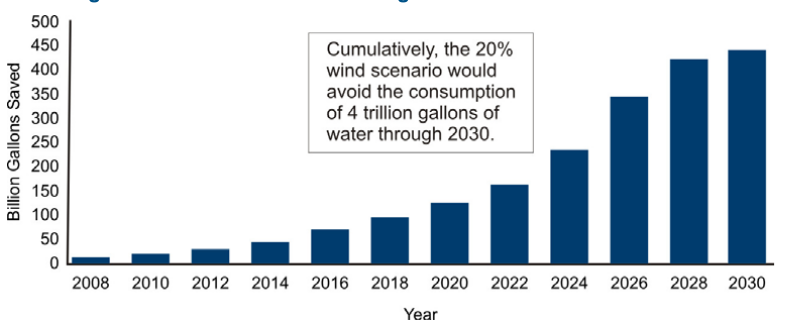
\includegraphics[width=\linewidth]{doe4.png}
                \caption{}
                \label{fig:do3}
        \end{subfigure}%
       \caption[$CO_2 \ \&$ Water Reduction]{ Propose reduction of (A) $CO_2$ emission (B) Water capacity, projected till 2030 with the goal towards ``20 \% Wind Scenario"}
\label{fig:smag}
\end{figure}

